%% TITOLO
\section{Ecosistemi Udibili}
\label{sec:Ecosistemi Udibili}
%% TESTO
% - proseguire partendo dagli articoli di Agostino Di Scipio, da Polveri Sonore,
% dalle analisi musicali come quelle di Makis Solomos. Discutere gli elementi del
% sistema e il loro ruolo in Audible Ecosystemics 2 + Codici Faust degli agenti.
% In coda al capitolo rimandare al codice completo in Appendice A e plot
% grafici di Faust in Appendice B -

Quello di cui abbiamo parlato fino ad ora nella tesi ha trattato la storia di 
un cambio di pardigma nella musica, in cui essenzialmente si è smesso di 
scrivere musica per strumenti interattivi con cui farla, e viceversa, 
e  si è passati invece al  comporre le interazioni tramite gli strumenti. \\
Le interazioni sistemiche che ho ritenuto importante affrontare all'interno di questa tesi 
come anticipato nell'abstract sono di due tipi, 
di sistemi che interagiscono con l’ambiente circostante appartenente al mondo fisico, 
e sistemi che interagiscono con il proprio ambiente nel mondo digitale. \\
Quello che si manifesta quando un sistema entra in interazione non distruttiva 
con l'ambiente circostante, che è il suo spazio vitale,  è un Ecosistema. 
In effetti nessun sistema è separabile e isolabile dall'ambiente circostante, 
a prescindere dal fatto che il suo spazio vitale sia nel mondo fisico o digitale. 
Proprio come ha mostrato Heinz Von Foerster non si può parlare di auto-organizzazione 
se non ci si riferisce essenzialmente a un ambiente che racchiude il sistema al suo interno. 
I lavori del ciclo Ecosistemico Udibile di Agostino di Scipio, in tal senso, 
trovano fondamento a partire da fenomeni e relazioni che possono esistere e manifestarsi solamente nell'ambiente 
circostante da cui prende vita il sistema, che in questo caso è proprio lo spazio acustico reale. 
Lavori come lo studio sul feedback, lo studio sul rumore di fondo, lo studio sulle risposte all'impulso, o
lo studio sul silenzio, sono in essenza dei sistemi che interrogano un determinato 
comportamento appartenente allo spazio acustico reale, delimitato in questi studi da una stanza,
per costruirne una storia di relazioni dove il sistema si osserva attraverso lo spazio fisico, 
si manifesta e vive solo attraverso di esso.
In questo senso l’interprete, lo spazio, e gli ascoltatori, 
divengono essi stessi parte integrante del sistema dove l’ascolto è 
parte dell’insieme delle cose e delle relazioni che lo costituisce. \\

\subsection{L'interazione Uomo-Macchina-Ambiente}
\label{sec:L'interazione Uomo-Macchina-Ambiente}

Qual'è dunque l'esigenza alla base del comporre le interazioni invece 
che limitarsi al comporre musica per strumenti interattivi? 
Superare la relazione uomo-macchina, iniziando a pensare allo sconfinato universo 
delle nuove possibilità della complessità.
Secondo Agostino Di Scipio, per l'appunto, alla possibilità che la macchina possa rappresentarsi, 
senza mediazione umana, attraverso l'ambiente circostante, \footcite{discipio_polverisonore_2016}
e dunque poi alla possibilità di stabilire un flusso di relazioni macchina-ambiente. 
Consentendo al performer la possibilità di potersi aprire ad un flusso di relazioni 
complesso fra uomo-macchina-ambiente dove le tre sono fortamente connesse e dipendenti 
l'una dall'altra.

\begin{center}
\vspace{0.5cm}
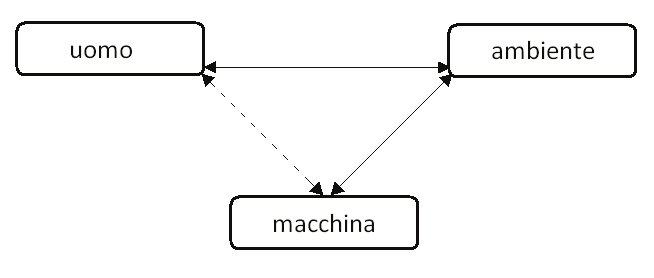
\includegraphics[width=8cm]{figures/uomo_macchina_ambiente.png} \\
{Interazione Uomo-Macchina-Ambiente \footcite{discipio_polverisonore_2016}} \\ 
\vspace{0.5cm}
\end{center}

\begin{center}
\vspace{0.5cm}
\textit{la mossa decisiva è: passare da un lavoro che mira a usare mezzi interattivi per creare forme sonore desiderate ad
un lavoro che mira a creare le interazioni desiderate e ad ascoltarne le tracce udibili. Nel secondo caso, si tratta
di progettare, implementare, e rendere operativo un reticolo di componenti interconnesse il cui comportamento
sonoro emergente si può chiamare musica.} \footcite{discipio_polverisonore_2016}
\vspace{0.5cm}
\end{center}

Il modo in cui andrò a discutere in questo capitolo la composizione di interazioni ecosistemiche, 
è ponendo il focus su un lavoro di Agostino Di Scipio, l’Ecosistemico Udibile n.2, studio sul feedback. 
Andando ad analizzare il ruolo e il compito dei singoli agenti all'interno del sistema 
che compongono nella loro totalità l'ecosistema e il brano. 

\subsection{Il Meccanismo LAR}
\label{sec:Il Meccanismo LAR}
Il feedback elettroacustico (effetto Larsen), che abbiamo visto
esser stata una delle risorse centrali dei primi compositori cibernetici,
è la condizione di partenza su cui Agostino Di Scipio opera per la costruzione degli Ecosistemi Udibili.
Addentrandoci verso una spiegazione più tecnica del feedback elettroacustico,
possiamo citare una definizione che Di Scipio ha esposto in un suo articolo
pubblicato presso la rivista Online: ECHO dell’ Orpheus Institute, in
Ghent. \footcite{di_scipio_relational_2022}

\begin{center}
\vspace{0.5cm}
\textit{A condenser microphone (M1) and a dynamic loudspeaker (L1) stand in the performance place
(S), few or several meters apart, maybe not too far from walls (or curtains, or other larger
surfaces). They are connected (through one or more amplification stages) to realize a very
basic electroacoustic chain: M1→L1→S. There’s no sound M1 should capture, though, no sound
source save the minimal, barely audible turbulence of the background noise, in a situation of
‘silence’. This ‘sound-of-nothing’ is amplified and heard through L1, whence it comes back in
S. \\
If amplification suffices, the L1 sound feeds back into M1 and the chain design closes onto
itself, making a ‘reinjection’ circuit – a feedback loop. The amplitude level, the
transductive technical features of M1 and L1, their relative distance, the distance from
walls, etc. – all of that (and much more) sets the actual feedback loop gain. With
not-too-high gain levels, what is engendered is an audible nuisance, a kind of ‘halo’: the
sound reinjection decays more or less rapidly, in a kind of badly sounding, spectrally uneven
reverb effect. With higher gain levels, the loop eventually enters a self-oscillatory regime,
it may ‘ring’ or ‘howl’, as is often said. Because of the iterated reinjection, the barely
audible but spectrally wide background noise accumulates in the loop and finally (quickly)
yields an increasingly louder sustained sound of narrower spectrum – this is often heard as a
peaking tone of definite pitch, or a tone cluster. That’s the Larsen effect: a self-sustaining
feedback resonance occasioned by a positive feedback loop (FB+) (‘positive’ here means greater
than unit gain).} \footcite{di_scipio_relational_2022}
\vspace{0.5cm}
\vspace{0.5cm}
\end{center}

\begin{center}
\vspace{0.5cm}

\includegraphics[width=8cm]{figures/larsen_feedback_scheme.png} \\
{Schema M1→L1→S \footcite{di_scipio_relational_2022}} \\ 
\vspace{0.5cm}
\end{center}

L'effetto Larsen: (dal nome del fisico Søren Absalon Larsen
che per primo ne scoprì il principio), detto anche feedback elettroacustico,
come abbiamo appena letto è un fenomeno di retroiniezione che tende idealmente 
ad un'accumulazione infinita, che viene limitata in realtà dalla saturazione dei sistemi 
che la generano (relativi alla potenza massima, all'amplificazione, nonché alla sensibilità dei
trasduttori e all'elasticità delle membrane). Che può però anche essere oltre al microfono, un
pick-up di uno strumento musicale elettrico, come una chitarra o un basso, o un trasduttore di
altra natura... 

\begin{center}
\vspace{0.5cm}
\textit{In common sound engineering practice, audible feedback phenomena are a nuisance, a problem one
should get rid of or substantially minimize. When direct level manipulation is not enough, one
resorts to hard-limiting circuits, ‘feedback killers’ and alike devices... 
In a different attitude, one may instead consider feedback as
a resource, a deliberately designed sound-making mechanism one can play with.} \footcite{di_scipio_relational_2022}
\vspace{0.5cm}
\vspace{0.5cm}
\end{center}

per utilizzare quindi il feedback come una
risorsa, evitando quindi questa sua crescita che porti alla saturazione dei sistemi, possiamo far calcolare
al computer in tempo reale tramite diverse tecniche di \textit{amplitude following} la stima dell'ampiezza
del segnale, ed utilizzare conseguentemente la \textit{feature extraction} come segnale di controllo
in retroazione al sistema di Feedback Elettroacustico.
Questo meccanismo di controbilanciamento del guadagno
del fenomeno è chiamato da Agostino Di Scipio col nome di LAR: \textit{Audio Feedback with Self-regulated Gain},
e che può essere implementato in DSP in diversi modi e configurazioni. \\

\begin{center}
\vspace{0.5cm}
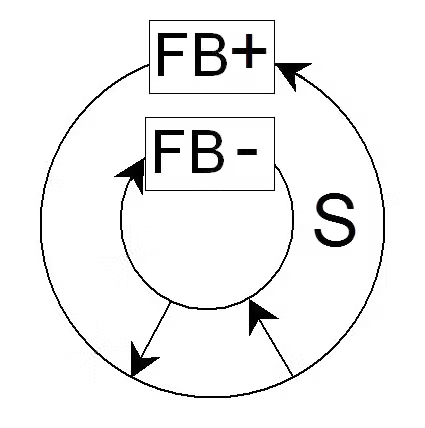
\includegraphics[width=8cm]{figures/controlled_larsen_feedback.png} \\
{Schema del meccanismo LAR \footcite{di_scipio_relational_2022}} \\ 
\vspace{0.5cm}
\end{center}

Ci sono poi, diversi modi per realizzare un algoritmo di controbilanciamento del feedback in tempo
reale nella tradizione della computer music.
Alcuni di questi possono riguardare controbilanciamenti nel dominio della frequenza,
con tecniche di filtraggio automatizzate (adattive) che
eliminino dallo spettro la presenza dell'autoscillazione prodotta dal Larsen \textit{Larsen Suppressors},
o come nel nostro caso d’interesse possono riguardare controbilanciamenti in ampiezza
automatizzati, che non permettano al Feedback di avere un guadagno troppo troppo elevato 
e giungere dunque ad uno stato di saturazione del sistema.
Nel secondo caso possono dunque essere implementati algoritmi di \textit{amplitude following} in
tempo reale con dei filtri che operano la media \textit{RMS}, a media mobile, 
filtri \textit{peakholder} che mantengono il valore di picco, o di altra natura. \\
Passiamo ora ad una parte più operativa, discutendo l'implementazione
di alcune di queste tecniche nel linguaggio di programmazione FAUST (Grame), 
l'ambiente in cui sono stati scritti i codici di tutti i lavori sviluppati 
per questa tesi e le relative compilazioni, diagrammi, softwares. \\
\footnote{FAUST (Grame) (Functional Audio Stream), 
è un linguaggio di programmazione specifico per il Digital Signal
Processing sviluppato da Yann Orlarey, Dominique Fober, e Stephane Letz nel
2002. Nello specifico, FAUST è un linguaggio di programmazione ad alto livello
scritto in C++, che permette di tradurre delle istruzioni date e create 
appositamente per il digital signal processing (DSP), in un largo raggio di linguaggi
di programmazione non specifici per il dominio dell’Audio Digitale.} \footcite{https://faust.grame.fr/}
Il modo più semplice per mantenere l’effetto Larsen in uno stato stazionario, è attraverso un
valore costante in retroazione che controbilancia l’ampiezza del segnale in ingresso; 
quando questa costante in ingresso nel filtro corrisponde al valore di picco maggiore 
di una finestra di campioni, il controbilanciamento in questione è chiamato tramite \textit{Peakholder}.
Il modo più semplice per implementare un Peakholder è tramite una finestra 
di campioni idealmente infinita IIR \textit{Infinite Impulse Response}. 
L’algoritmo presenta comunque alcuni problemi: non possedendo
una funzione di smoothing del segnale, si verificano problemi di segnali di differenza a banda
molto larga che possono generare aliasing e contributi spuri che tendono a permanere nel
segnale complessivo.




